\documentclass[twoside]{report}
\usepackage[italian]{babel}
\usepackage[utf8]{inputenc}
\usepackage{amsmath}
\usepackage{amsthm}
\usepackage{amsfonts}
\usepackage{amssymb}
\usepackage{cancel}
\usepackage[margin=1in]{geometry}
\usepackage{hyperref}
\usepackage{bookmark}
\usepackage{setspace}
\usepackage{titlesec}
\usepackage{hyperref}
\usepackage{graphicx}
\usepackage{fancyhdr}
\usepackage{float}
\usepackage{wrapfig}


\graphicspath{{./images/}}

\newcommand{\figref}[1]{\figurename~\ref{#1}}

\setlength{\parskip}{0pt}
\titlespacing*{\subparagraph}{1.25em}{0em}{0.35em} 

\makeatletter
\renewenvironment{abstract}{%
    \if@twocolumn
        \section*{\abstractname}%
    \else
        \begin{center}%
            {\bfseries \abstractname\vspace{-.5em}\vspace{\z@}}%
        \end{center}%
        \small
        \begin{quotation}
    \fi}
    {\if@twocolumn\else\end{quotation}\fi}
\makeatother

\fancypagestyle{chapterInit}{%
    \fancyhf{}
    \renewcommand{\headrulewidth}{0pt}
    \fancyfoot{}
    \fancyfoot[LE,RO]{\thepage}
    \fancyfoot[LO,RE]{"Appunti di Introduction to Computer and Network Security" di Luca Facchini}
    \renewcommand{\footrulewidth}{0.4pt}
}
\fancypagestyle{stdPageS}{
    \fancyhead{}
    \fancyhead[RO,LE]{\leftmark}
    \fancyfoot{}
    \fancyfoot[LE,RO]{\thepage}
    \fancyfoot[LO,RE]{"Appunti di Introduction to Computer and Network Security" di Luca Facchini}
    \renewcommand{\footrulewidth}{0.4pt}
}

\addtocontents{toc}{\protect\thispagestyle{stdPageS}}

\title{Appunti di Introduction to Computer and Network Security}
\author{Luca Facchini (mat. 245965)}
\date{A.A. 2024/2025}

\hypersetup{
    pdfauthor={Luca Facchini},
    pdftitle={Appunti di Introduction to Computer and Network Security},
    pdfsubject={Appunti del corso di Introduction to Computer and Network Security tenuto dal prof. Raniese Silvio presso l'Università degli Studi di Trento nell'anno accademico 2024/2025.},
    pdfkeywords={Computer Security, Network Security, Introduction to Computer and Network Security, UniTN, Università degli Studi di Trento},
    pdfproducer={LaTeX},
    pdfcreator={pdflatex},
}

\begin{document}
    \begin{titlepage}
        \centering  % Center everything on the title page
        {\Huge\textbf{Appunti di Introduction to Computer and Network Security}} \\[1cm] % Title
        \vspace{0.5cm}
        
        {\Large Luca Facchini} \\ % Author name
        \vspace{0.3cm}
        {\large Matricola: 245965} \\[2cm] % Additional author info
        
        {\large Corso tenuto dal prof. Raniese Silvio} \\[0.3cm] % Course information
        {\large Università degli Studi di Trento} \\[1.5cm]
        
        {\large A.A. 2024/2025} \\[3cm] % Academic year
        
        % Abstract section with spacing control
        \vfill
        \begin{abstract}
            Appunti del corso di Introduction to Computer and Network Security tenuto dal prof. Raniese Silvio presso l'Università degli Studi di Trento nell'anno accademico 2024/2025.
        \end{abstract}
        
        \vfill  % Pushes the content to the center vertically
    \end{titlepage}
    \pagestyle{stdPageS}
    \begingroup
        \setcounter{tocdepth}{2}
        \tableofcontents
    \endgroup
    \chapter{Basic Notions - Nozioni Base}
\thispagestyle{chapterInit}
\section{The CIA Triad}
\label{sec:ciaTriad}
    \subsection{Introduzione}
    \paragraph{L'acronimo} L'acronimo CIA in inglese sta per \textbf{Confidentiality}, \textbf{Integrity} e \textbf{Availability}. Questi tre concetti sono alla base della sicurezza informatica e della protezione dei dati.  
        \subparagraph{Confidentiality - Riservatezza}
        \label{subPar:confidentiality}
            Il principio della Riservatezza prescrive che i non autorizzati non devono poter accedere ai dati e i dati sono visibili solo a chi è autorizzato a vederli.
        \subparagraph{Integrity - Integrità}
        \label{subPar:integrity}
            Il principio di Integrità prescrive che i dati non devono essere modificati se non da persone autorizzate a farlo, i tentativi di modifica non autorizzati devono essere rilevati e prevenuti.
        \subparagraph{Availability - Disponibilità}
            Il principio della Disponibilità prescrive che i dati non devono essere mantenuti inaccessibili ed inoltre bisogna permettere l'accesso agli autorizzati alle informazioni e ai servizi.
    \subsection{In Pratica}
        \paragraph{Confidentiality - Riservatezza}
            L'accesso alle informazioni riservare può essere:
            \subparagraph{Intenzionale} Quando un intruso cerca di accedere a dati sensibili.
            \subparagraph{Non Intenzionale} Quando un utente autorizzato accede a dati sensibili senza volerlo causato dal fatto che chi detiene i dati non è competente e/o non gli importa della sicurezza.
        
            Come garantire la riservatezza:
            \subparagraph{Crittografia} La \textbf{crittografia} è una tecnica che permette di limitare l'accesso ai dati solo a chi possiede la chiave per decifrarli (e quindi è autorizzato).
            \subparagraph{Access Control} Il \textbf{controllo degli accessi} è una parte integrante per mantenere la \textbf{riservatezza}, ciò andando a gestire quali utenti possono accedere a quali risorse.
        \paragraph{Integrity - Integrità}
            Per garantire l'integrità bisogna prevenire la modifica e/o la distruzione, inoltre bisogna assicurare informazioni autentiche e non invalidate.

            Inoltre ulteriore prescrizione è quella di individuare anche le cosiddette "minute changes" ovvero le modifiche minime che possono essere fatte ai dati per alterarne il significato. 
            
            L'integrità può essere anche di tipo \textbf{data integrity} ovvero la garanzia che i dati siano corretti e completi, oppure di tipo \textbf{system integrity} ovvero la garanzia che il sistema sia protetto da attacchi e che funzioni correttamente.

            L'itemize può essere compromessa da:
            \begin{itemize}
                \item errore umano
                \item attacchi come malware distruttivi e ransomware
            \end{itemize}
            Come garantire l'integrità:
            \subparagraph{Version Control} Il \textbf{controllo delle versioni} assieme agli \textbf{audit trails} permettono ad una organizzazione di garantire la veridicità dei dati.
            \subparagraph{Compliance requirements} I \textbf{requisiti di conformità} sono regole e normative che un'organizzazione deve seguire per garantire l'integrità dei dati.
        \paragraph{Availability - Disponibilità}
            Le violazioni alla disponibilità includono:
            \begin{itemize}
                \item Fallimento dell'infrastruttura 
                \item Overload dell'infrastruttura
                \item Blackout
                \item Attacchi come DDoS
            \end{itemize}
            Come garantire la disponibilità:
            \subparagraph{Backup} Bisogna sempre avere un piano di \textbf{backup} per mantenere disponibile in caso di disastro, attacco o altre minacce si verificassero.
            \subparagraph{Cloud} Il \textbf{cloud} è una soluzione per garantire la disponibilità dei dati, in quanto i dati sono replicati su più server e quindi in caso di guasto di uno di essi i dati sono comunque disponibili.
        
\section{Security Policy, Mechanism, Service}
    \subsection{Security Policy}
            \subsubsection{Definizione}
                Una \textbf{security policy} è un insieme di regole e requisiti stabilita da una azienda che definisce l'uso accettabile delle informazioni e dei servizi, inoltre il livello indica il livello di confidenzialità, integrità e disponibilità delle informazioni.
            \subsubsection{Esempi}
                Un esempio di possibili regole di una \textbf{security policy} potrebbero essere:
                \begin{itemize}
                    \item I dipendenti devono completare il corso su sicurezza informatica e accettare la policy di sicurezza.
                    \item I visitatori dell'azienda devono essere accompagnati da un dipendente autorizzato in tutti i momenti, questo dipendente deve mantenere i visitatori in una area appropriata senza dati sensibili
                    \item I dipendenti devono mantenere una "scrivania pulita" dunque senza lasciare documenti sensibili accessibili e incustoditi.
                    \item I dipendenti devono usare una password sicura e queste non devono essere usate in altri servizi esterni.
                    \item Gli ex-dipendenti non devono mantenere alcun dato dell'azienda.
                \end{itemize}
    \subsection{Security Service}
            \subsubsection{Definizione} La capacità di supportare uno o più dei requisiti di sicurezza (Confidentiality, Integrity, Availability) e.s.: gestione chiavi, controllo accessi, autenticazione.
                Come già detto i \textbf{Security Services} implementano uno o più \textbf{Security Mechanism} che servono per far rispettare la \textbf{Security Policy}.
            \subsubsection{Esempi}
                \paragraph{HTTP(S)}
                    \subparagraph{HTTP} Se si sua il protocolla \textbf{HTTP} per la trasmissione dei dati qualsiasi informazione trasmessa può venire intercettata da hacker nel mezzo.
                    \subparagraph{HTTPS} Per ovviare a questo problema si usa il protocollo \textbf{HTTPS} che è una versione sicura di \textbf{HTTP} che usa la crittografia per proteggere i dati, in questo modo i dati trasmessi vengono cifrati e se intercettati non possono essere letti.
                \paragraph{Access Control}
                    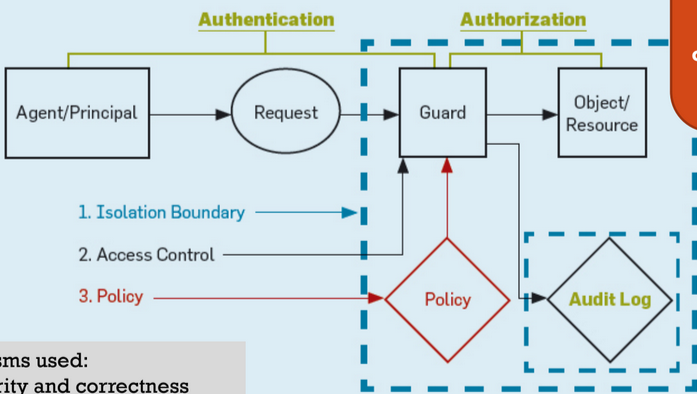
\includegraphics[height=12.5em]{01/accessControlSchema.png}
                    \subparagraph{Audit Log} è un registro importante che registra tutte le richieste di accesso ai dati e se la richiesta è stata accettata o rifiutata, in questo modo si può monitorare se una richiesta che è stata fatta ha avuto un risultato non aspettato e quindi che vadano modificate le \textbf{policy}.
    \subsection{Security Mechanism}
    \label{subsec:securityMechanism}
        \subsubsection{Definizione} Un \textbf{security mechanism} un dispositivo o funzione designato per provvedere uno o più servizi di sicurezza classificate in termini di potenza
            
            Inoltre è l'implementazione della \textbf{security policy}
        \subsubsection{Esempi}
    \subsection{Come si relazionano}
        In conclusione i \textbf{Security Services} implementano uno o più \textbf{Security Mechanism} che servono per far rispettare la \textbf{Security Policy}.
        
        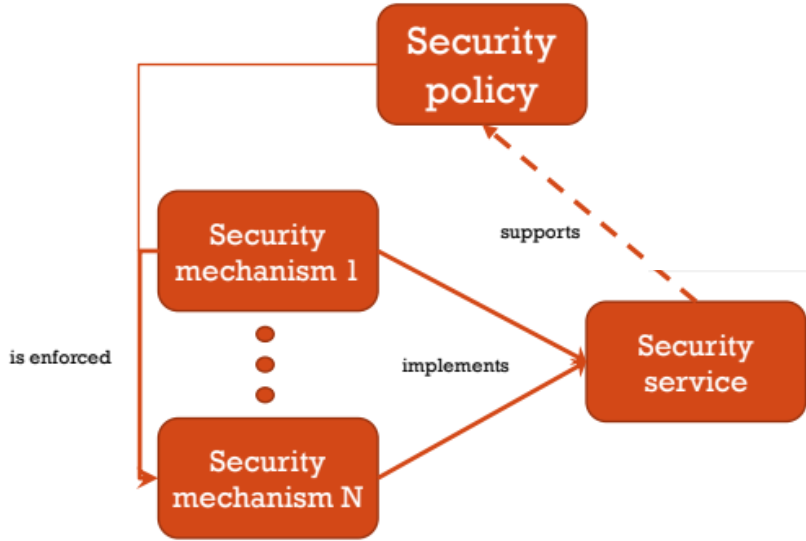
\includegraphics[height=10em]{01/schemaSecurity.png}
\section{CIA, Security Violation, and Mitigation}
    \paragraph{} La triade CIA non è solo essenziale per rendere sicuri i dati ma aiuta anche a capire cosa è andato storto nel caso di una \textbf{security violation}
    \subsection{Attacco Ransomware}
        \paragraph{L'arttacco}
            Nel caso di un attacco ransomware i dati vengono tenuti in ostaggio e la vittima viene ricattata con la pubblicazione di dati personali o il mancato accesso ad essi fino a che un riscatto non viene pagato.

            Questo attacco cripta i dati rendendoli inaccessibili e per ripristinarli è necessaria una chiave di decodifica, i pagamenti solitamente vengono eseguiti in crypto valute poco tracciabili.

            Questo genere di attacco viola la \textbf{confidentiality} e la \textbf{availability} dei dati.
        \paragraph{Mitigation}
            Per mitigare il rischio (che comunque non può essere eliminato) è utile procedere con un approccio \textbf{Zero Thrust} ovvero un "protocollo" che richiede che tutti gli utenti all'interno e all'esterno della rete aziendale siano autenticati e che la connessione è continuamente validata, prima di consentire accesso a applicazioni e dati.

\section{Risk}
    \paragraph{} Non esiste un sistema sicuro, esistono solo diversi livelli di insicurezza, si punta sempre ad ottenere il miglior livello di sicurezza possibile con il budget a disposizione.
    \subsection{Vulnerability}
        \subsubsection{Definizione}
            Una \textbf{vulnerabilità} è una debolezza in un sistema informativo, un sistema di sicurezza, nei controlli interni o nell'implementazione di questi. Questa debolezza può essere sfruttata o compromessa da una minaccia alla sicurezza.
        \subsubsection{Examples}
            Un esempio di \textbf{vulnerabilità} è una backdoor nascosta nel software e/o hardware, oppure dei bug non conosciuti di un software, o anche delle password deboli.
    \subsection{Threat}
        \subsubsection{Definizione}
            Qualunque circostanza o evento con il potenziale per causare perdite o danni a: operazioni dell'azienda, risorse o individui che possono accedere a tali risorse tramite un accesso non autorizzato, distruzione, pubblicazione, modifica e/o DoS. Inoltre un \textbf{threat} è un potenziale attacco che sfrutta una \textbf{vulnerabilità} del sistema.
        \subsubsection{Examples}
                Un esempio di \textbf{threat} sono:
                \begin{itemize}
                    \item Hacker:
                        \begin{itemize}
                            \item Trova e/o \textbf{sniff} una password.
                            \item Una il \textbf{social engineering} per ottenere informazioni sensibili e password.
                            \item Occupa le risorse di sistema con richieste inutili (attacchi DoS).
                        \end{itemize}
                    \item Virus e worms:
                        \begin{itemize}
                            \item I \textbf{virus} sono programmi auto replicanti che richiedono una azione dell'utente per essere attivati, esempio ne è una Email, un allegato o un link o un Floppy/CD/USB infetto.
                            \item I \textbf{worms} sono programmi auto replicanti che non richiedono una azione dell'utente per essere attivati, esempio ne è un worm che sfrutta una vulnerabilità di un sistema operativo.
                        \end{itemize} 
                \end{itemize}
    \subsection{Attack}
        \subsubsection{Definizione} Un \textbf{attacco} è un qualsiasi attività dannosa che prova a raccogliere, degradare, negare o distruggere informazioni o servizi. Può anche manifestarsi sotto un tentativo di ottenere un accesso ad una risorsa alla quale non si ha diritto 
    \subsection{Risk}
        \subsubsection{Definizione}
            Il \textbf{rischio} è la \textbf{probabilità} che una particolare \textbf{minaccia} \textbf{sfrutti} una particolare \textbf{vulnerabilità}.Il \textbf{rischio} è inoltre una misura di quanto una particolare circostanza o evento possa essere potenzialmente minacciato ed è tipicamente in funzione di: 
            \begin{enumerate}
                \item L'impatto che questa circostanza o evento potrebbe avere
                \item La probabilità che questa circostanza o evento si verifichi
            \end{enumerate}
        \subsubsection{Riassumendo}
            Riassumendo le \textbf{minacce} sono una combinazione di \textbf{intento} e \textbf{capability} di un attacco con successo. Invece le \textbf{vulnerabilità} sono caratterizzate da quanto è facile \textbf{identificarle} e \textbf{sfruttarle}.
            
            C'è da dire che l'impatto di un attacco deve essere valutato dal punto di vista di ogni soggetto coinvolto, ad esempio un attacco che compromette la privacy di un singolo individuo può avere un impatto molto diverso se lo si guarda dal punto di vista dell'individuo o dell'azienda.
        \subsubsection{Risk Matrix}
            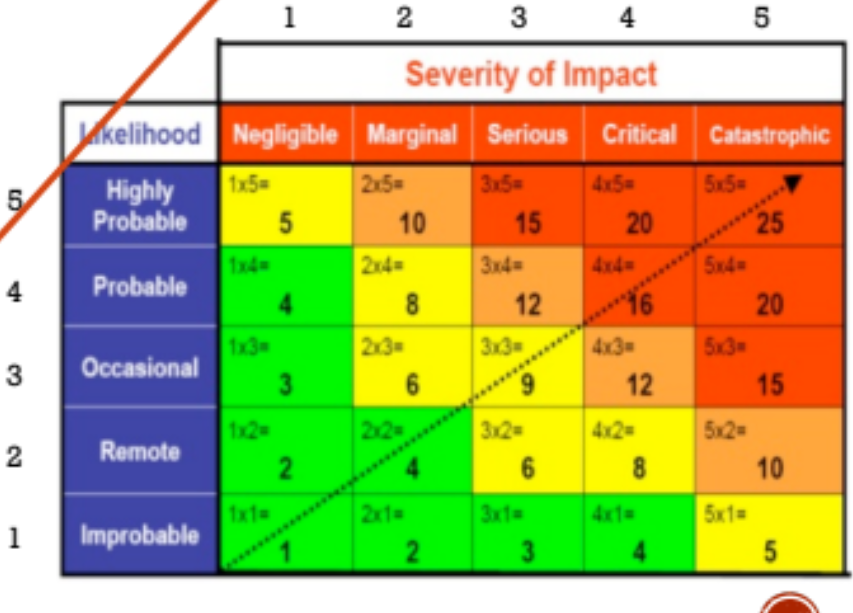
\includegraphics[height=10em]{01/riskMatrix.png}
            
            La presente matrice è una rappresentazione grafica del rischio, in cui si valuta la probabilità di un attacco e l'impatto che questo avrebbe, solitamente un rischio per essere accettabile deve avere un valore risultante tra basso (1-4) e medio-basso (5-9), i valori quali medio-alto (10-14) e alto (15-25) sono considerati inaccettabili e quindi devono essere mitigati abbassando la probabilità di attacco e/o l'impatto che questo avrebbe.

\section{Fine della diffusione degli attacchi}
    \paragraph{Generalmente} Il rischio è causato dunque dalla somma di una minaccia e una vulnerabilità, la minaccia è la capacità di sfruttare una vulnerabilità per causare un danno. 
    \paragraph{Pianizifazione} Quando si studiano i rischi sia prima che dopo un attacco bisogna considerare che se la \textbf{Minaccia - Threat} riesce a sfruttare la \textbf{Vulnerabilità - Vulnerability} allora si ha un \textbf{Rischio - Risk} se questo risulta inaccettabile allora si deve procedere con la \textbf{Mitigazione - Mitigation} del rischio, ciò riduce la \textbf{Minaccia - Threat} e il ciclo riprende fino a quando il \textbf{Rischio residuo - Residual Risk} è accettabile.

\section{Security \& Human Factor - Sicurezza \& Fattore Umano}
    Il fattore umano è uno dei fattori più importanti nella sicurezza informatica, infatti la maggior parte degli attacchi sono causati da password poco sicure o da una mancata preparazione degli utenti.
    \subsection{Passwords}
        C'è chi dice che le password andrebbero trattate come la biancheria intima, ovvero:
        \begin{itemize}
            \item Cambiate regolarmente - magari senza usare un pattern
            \item Non condivise con nessuno - nemmeno con colleghi o familiari
            \item Non lasciate sulla scrivania - non scritte su post-it o in chiaro
        \end{itemize}
    \subsection{Security}
        Ogni persona che ha accesso ad un sistema informatico è un potenziale punto di attacco, quindi è importante che ogni utente sia formato sulla sicurezza, ogni utente al suo livello a partire dall'utente base che necessita di una formazione base fino ad arrivare all amministratore di sistema che necessita di una formazione più avanzata.
    \chapter{Authentication I: Passwords \& co}
\thispagestyle{chapterInit}
\section{User Authentication \& Digital Identity - Autenticazione e Identità Digitale}
    \label{sec:user-authentication}
    \subsection{Introduzione e Definizioni}
        \begin{description}
            \item[Identità] è un insieme di attributi relazionati ad una entità
            \item[Attributo] è una caratteristica o proprietà di una entità ch e può essere usata per descriverne lo stato, apparenza o ogni altro aspetto.  
            \item[Identità digitale] è ua identità i quali attributi sono conservati e trasmessi in forma digitale 
        \end{description}
        Ma perché la identità digitale è importante? In pratica questa può essere una soluzione per diversi aspetti che i governi mondiali vorrebbero risolvere.
    \subsection{Digital Identity Lifecycle - Ciclo di Vita dell'Identità Digitale}
        \begin{description}
            \item[Creazione] L'identità viene creata, in genere da un ente di certificazione che assicura l'identità dell'utente e fornisce/chiede una forma di accesso per riconoscere in futuro l'utente. Viene creato un ID univoco per l'utente
            \item[Autenticazione] L'identità viene autenticata tramite il metodo concordato in fase di creazione
            \item[Autorizzazione/ Accesso] L'utente ha accesso a risorse e servizi in base ai permessi assegnati, i dati necessari dell'utente vengono trasmessi dall'ente di certificazione al servizio.
            \item[Cancellazione o Disattivazione] L'identità viene cancellata o disattivata quando non è più necessaria e i dati devono essere cancellati dopo un certo periodo di tempo per garantire la privacy dell'utente.
        \end{description}
        \subsubsection{Enrollment / On-Boarding - Creazione}
            La fase di creazione di una utenza porta un \textbf{Applicant} a diventare un \textbf{Subscriber} tramite una serie di passaggi:
            \begin{description}
                \item[Resolution] Vengono raccolti gli \textbf{attributi} essenziali dell'utente (nome, indirizzo, data e luogo di nascita, \dots) vengono ora raccolti anche due documenti di identità (patente, passaporto, C.I.,\dots) - ora l'utente viene distinto univocamente su un contesto
                \item[Validation] Gli \textbf{attributi} raccolti vengono validati sulla base di \textbf{prove} tramite una fonte autorevole- gli attributi vengono ora associati ad una persona fisica 
                \item[Verification] Le \textbf{prove} vengono verificate, in questo punto si verifica la corrispondenza tra le diverse foto, viene mandato un codice ai contatti per verificare che siano i suoi, etc - l'utente viene ora confermato e la sua identità è certificata 
            \end{description}
            \paragraph{Identity Assurance Levels - Livelli di Assicurazione dell'Identità}
                \begin{description}
                    \item[IAL1] GLi attributi, se presenti, vengono auto-dichiarati, o considerati come tali
                    \item[IAL2] Una persona o di remoto o in presenza, verifica gli attributi
                    \item[IAL3] Gli attributi vengono verificati da una persona autorizzata e i documenti fisici vengono esaminati
                \end{description}  
        \subsubsection{Authentication - Autenticazione}
            \paragraph{Definzione} L'\textbf{autenticazione} è il processo di verifica dell'identità di un utente, processo o dispositivo.

            Il \textbf{richiedente} deve dimostrare al \textbf{verificante} che è chi dice di essere.
            \paragraph{Base} Quando esegui il login solitamente inserisci un \textbf{username} e una \textbf{password} che vengono confrontati con quelli memorizzati nel sistema.

            L'autenticazione tramite \textbf{password} è molto diffusa e semplice da implementare.
\section{An Introduction to Passwords - Introduzione alle Password}
    \subsection{User Authn - Autenticazione Utente}
        Quando esegui il login inserisci un \textbf{username} per annunciare chi sei e una \textbf{password} per dimostrare chi dici di essere, questo tipo di autenticazione si chiama \textbf{user authn} ovvero il processo di verifica dell'identità di un utente.
        \subsubsection{Entollment - Creazione}
            Le \textbf{password} dovrebbero essere conosciute solo dall'utente e dal sistema. Spesso però, soprattutto nelle grandi aziende, le password vengono mandata via mail o scritte dall'utente su una pagina web. In questi casi da chi potrebbe essere intercettata la password?
        \subsubsection{La teoria rispetto alla realtà}
            Le password hanno dominato il mondo dell'informatica sin dall'avvento dei computer, ma da allora la richiesta verso queste è che siano più sicure ma allo stesso tempo più "User Friendly", siamo in ricerca di alternative ma per ora delle proposte alternative come \textit{criteri di complessità} ma studi hanno rilevato che spesso non vengono rispettati e/o che non sono efficaci. 
    \subsection{Password Security - Sicurezza delle Password}
        All'inizio di internet le password venivano conservate in file appositi in chiaro, ma questo comportava un rischio molto alto, infatti se un attaccante riusciva ad accedere a quel file poteva facilmente accedere a tutte le password.

        \subsubsection{Hashing}
            Per risolvere questo problema si è pensato di "\textbf{hash-are}" le password, ovvero di applicare una funzione di hash alla password e conservare il risultato. In questo modo se un attaccante accede al file delle password non può risalire alla password originale.
            \paragraph{Proprietà della funzione di hash}
                Una funzione di hash ottimale dovrebbe avere le seguenti proprietà:
                \begin{description}
                    \item[Deterministica] dato un input la funzione restituisce sempre lo stesso output
                    \item[Rapida] la funzione deve essere veloce da calcolare
                    \item[Difficile da invertire] data l'output è difficile risalire all'input
                    \item[Biettiva] due input diversi devono avere output diversi
                    \item[Lunghezza fissa] l'output deve avere una lunghezza fissa indipendentemente dalla lunghezza dell'input
                \end{description}
                Molto spesso però capita che i bit disponibili per l'hash siano limitati rispetto a tutti i possibili input, per questo motivo si è cercato di creare funzioni di hash che generano due output uguali solo in rarissimi casi, inoltre si aggiunge a questo che per input simili l'output sia molto diverso.
            \subsubsection{Crack of Passwords}
                In caso di un "leak" di password che sono state opportunamente codificate con una funzione di hash, un attaccante può tentare di decifrarle ma questo è molto difficile. Questo diventa più semplice se vengono usate password poco sicure e/o comuni. infatti si stimi che per  trovare una password da 8 caratteri composti da lettere minuscole e numeri ci vogliano "solo" 155€ su una istanza di AWS.
        \subsection{Hash \& Salt}
            Per rendere più difficile il lavoro degli attaccanti si è pensato di aggiungere un \textbf{salt} alle password, ovvero un valore casuale che viene aggiunto alla password prima di calcolare l'hash. Questo rende più difficile per l'attaccante decifrare la password.
\section{Multi Factor Authentication - Autenticazione a più fattori}
\label{sec:mfa}
    \subsection{Definizione}
        L'autenticazione a più fattori è un metodo di autenticazione che richiede l'uso di più metodi di autenticazione per verificare l'identità di un utente.
    \subsection{Fattori di Autenticazione}
        I fattori di autenticazione sono:
        \begin{description}
            \item[Qualcosa che sai] (password, PIN, \dots)
            \item[Qualcosa che hai] (smartphone, token, \dots)
            \item[Qualcosa che sei] (impronte digitali, riconoscimento facciale, \dots)
        \end{description}
        \subsubsection{Vantaggi/Svantaggi quello che sai}
            \paragraph{Vantaggi}
                \begin{itemize}
                    \item Facile da implementare - non richiede hardware aggiuntivo
                    \item Facile da usare - Basta ricordare la password
                    \item Facile da resettare se dimenticato - basta fare il reset della password
                \end{itemize}
            \paragraph{Svantaggi}
                \begin{itemize}
                    \item Facile da rubare - se un attaccante riesce a scoprire la password può accedere al sistema 
                    \item Facile da dimenticare - se la password è complessa è facile dimenticarla
                    \item Facile da indovinare - se la password è semplice ed è stata usata in altri contesti è facile indovinarla
                \end{itemize}
        \subsubsection{Vantaggi/Svantaggi quello che hai}
            \paragraph{Vantaggi}
                \begin{itemize}
                    \item Difficile da rubare - se un attaccante non ha il dispositivo non può accedere al sistema
                    \item Difficile da indovinare - se il dispositivo è protetto da PIN o password è difficile indovinare l'accesso
                    \item Difficile da clonare - se il dispositivo è protetto da un token è difficile clonarlo inoltre la parte di autenticazione è fatta dal dispositivo stesso e non dal sistema
                \end{itemize}
            \paragraph{Svantaggi}
                \begin{itemize}
                    \item Facile da perdere - se il dispositivo viene perso l'utente non può accedere al sistema
                    \item Difficile da resettare - se il dispositivo viene perso l'utente deve contattare l'amministratore per resettare l'accesso
                    \item Costoso - i dispositivi possono essere costosi 
                \end{itemize}
        \subsubsection{Vantaggi/Svantaggi quello che sei}
            \paragraph{Vantaggi}
                \begin{itemize}
                    \item Difficile da rubare - le impronte digitali o il riconoscimento facciale sono unici e difficili da rubare
                    \item Difficile da indovinare - è difficile indovinare le impronte digitali o il riconoscimento facciale
                    \item Difficile da clonare - è difficile clonare le impronte digitali o il riconoscimento facciale
                \end{itemize}
            \paragraph{Svantaggi}
                \begin{itemize}
                    \item Se il fattore viene compromesso non può essere cambiato - se le impronte digitali vengono rubate non possono essere cambiate
                    \item Costoso - i dispositivi possono essere costosi
                    \item Non sempre preciso - il riconoscimento facciale può essere ingannato
                \end{itemize}
        \subsubsection{PSD2 Compliance}
            \paragraph{Cos'è PSD2} La \textbf{PSD2} è una direttiva europea che regola i servizi di pagamento e che richiede l'autenticazione a più fattori per i pagamenti online. Questo per ridurre il rischio di frodi.
            \paragraph{How to comply MFA in PSD2} Una idea sarebbe quella di includere nella challenge anche i dati della particolare transazione come:
                \begin{itemize}
                    \item L'identificativo del destinatario della transazione
                    \item L'importo della transazione
                    \item L'instante nella quale la transazione è stata inizializzata
                    \item \dots
                \end{itemize}
            Purtroppo però ciò non è abbastanza in quanto i dati sopra indicati possono essere ricavati dal contesto il che rende la challenge prevedibile.
    \subsection{FIDO: Phishing Resistant Authentication}
        \subsubsection{Cos'è FIDO}
            \textbf{FIDO (Fast Identity Online)} è un insieme di standard aperti per l'autenticazione a più fattori che mira a ridurre il rischio di phishing. Il suo scopo è quello di assicurare una \textbf{autenticazione forte} e di \textbf{ridurre l'uso di password}.
        \subsubsection{Come funziona}
            \begin{enumerate}
                \item Viene chiesto all'utente di scegliere un ente FIDO
                \item L'utenti sblocca il dispositivo FIDO usando un'impronta digitale, un pulsante su un dispositivo di secondo fattore, un PIN o un qualsiasi altro metodo di autenticazione supportato
                \item Il dispositivo crea una chiave pubblica e una chiave privata univoca per il dispositivo, il servizio online e l'utente
                \item La chiave pubblica è inviata al servizio online ed associata all'account dell'utente
                \item Il servizio online chiede all'utente di autenticarsi con il dispositivo precedentemente registrato
                \item L'utente sblocca il dispositivo FIDO usando lo stesso metodo di autenticazione usato in precedenza
                \item Il dispositivo FIDO usa l'account dell'utente identificato per inviare la corretta chiave al servizio online
                \item Infine il dispositivo invia la challenge ricevuta dal servizio online firmata con la chiave privata e il servizio online verifica la firma con la chiave pubblica, l'utente è autenticato.
            \end{enumerate}
\section{Outsourcing Authentication}
    \label{sec:outsourcing-authentication}
    \subsection{Definizione}
        L'outsourcing dell'autenticazione è il processo di affidare l'autenticazione degli utenti ad un servizio esterno, spesso chiamato \textbf{Identity Provider}. Questo servizio si occupa di verificare l'identità dell'utente e di inviare un token di autenticazione al servizio che richiede l'autenticazione. Esempio in italia per l'accesso ai servizi pubblici si usa SPID.
    \subsection{Che problema risolve}
        L'outsourcing dell'autenticazione risolve diversi problemi:
        \begin{description}
            \item[Sicurezza] L'Identity Provider è specializzato in autenticazione e può offrire un livello di sicurezza più alto
            \item[User Experience] L'Identity Provider può offrire un'esperienza utente migliore in quanto l'utente non deve ricordare le password per ogni servizio ma solo quella dell'Identity Provider - SSO
            \item[Compliance] L'Identity Provider può aiutare a rispettare le normative sulla privacy e la sicurezza
        \end{description}
    \subsection{La soluzione}
        L'outsourcing dell'autenticazione è delegato ad una terza parte, l'\textbf{Identity Provider}, che si occupa di verificare l'identità dell'utente e di inviare le informazioni di autenticazione al servizio che richiede l'autenticazione. A questo punto il servizio invia all'utente un token di autenticazione che può essere usato per accedere al servizio senza dover inserire nuovamente le credenziali del SSO.
    \subsection{Potenziali Problemi}
        L'outsourcing dell'autenticazione può comportare alcuni problemi:
        \begin{description}
            \item[Single Point of Failure] Se l'Identity Provider è compromesso tutti i servizi che usano l'Identity Provider per l'autenticazione sono compromessi
            \item[Privacy] L'Identity Provider può raccogliere informazioni sull'utente e sulle sue abitudini di navigazione
        \end{description}
    \chapter{Cryptography Introduction}
\section{Cryptosystem}
    \paragraph{Definizione} Un \textbf{cryptosystem} è una tupla di 5 elementi (E,D,M,K,C):
    \begin{description}
        \item[E] è un \textit{algoritmo di cifratura}
        \item[D] è un \textit{algoritmo di de-cifratura}
        \item[M] è un insieme di \textit{messaggi in chiaro}
        \item[K] è un insieme di \textit{chiavi}
        \item[C] è un insieme di \textit{messaggi cifrati}
    \end{description}
    In modo astratto i punti \textbf{E} e \textbf{D} possono essere espresse come funzioni:
    $$
        \begin{aligned}
            E: M \times K \rightarrow C \\
            D: C \times K \rightarrow M
        \end{aligned}
        \qquad D(E(m,k),k) = m
    $$
    Nella criptografia base ogni chiave $ k \in K $ può essere usata per cifrare e de-cifrare i messaggi, nella criptografia simmetrica la chiave è la stessa per entrambi i processi, mentre nella criptografia asimmetrica le chiavi sono diverse.
    \paragraph{Quali componenti sono pubbliche?} Solitamente non abbiamo necessità di mantenere segrete le funzioni \texttt{E} e \texttt{D} o il messaggio cifrato \texttt{C}, quello che davvero deve essere segreto è la chiave \texttt{K}. Il motivo per il quale le funzioni non devono essere segrete è che il sistema deve essere pubblico e quindi tramite processi di \textit{reverse engineering} è possibile ricavare le funzioni (es: il sistema di cifratura di un DVD è stato ricavato tramite \textit{reverse engineering} dopo solo due giorni).
    \subsection{Why Cryptography?}
        \paragraph{Sicurezza} La crittografia è usata nei \hyperref[subsec:securityMechanism]{\textbf{meccanismi di sicurezza}} per garantire \hyperref[subPar:confidentiality]{\textbf{confidenzialità}} nascondendo il contenuto dei messaggi, \hyperref[subPar:integrity]{\textbf{integrità}} provvedendo al controllo di integrità tramite funzioni di \textbf{hash} e \textbf{la verifica dell'origine} dei dati tramite firme digitali verificabili da una fonte autorevole.
    \subsection{Cryptography on rented servers}
        \paragraph{Problema} Se si usa un server di terze parti per conservare dati, ad esempio su un database, è possibile che il proprietario del server possa accedere ai dati in chiaro. Per evitare ciò si può cifrare i dati prima di inviarli al server, in modo che il proprietario non possa leggerli, ciò comporta però un aumento del carico computazionale lato client in quanto tutti i dati prima di essere letti devono essere de-cifrati, per questo esistono meccanismi di ricerca su dati cifrati che permettono di effettuare ricerche su dati cifrati senza de-cifrarli, una volta trovati i dati desiderati si de-cifrano solo quelli.
    \subsection{Come definiamo "Computazionalmente sicuro" nelle comunicazioni}
        \paragraph{Definzizione} Definiamo un sistema di comunicazione \textbf{Computazionalmente sicuro} quando la decifrazione di un messaggio cifrato senza conoscere la chiave è molto difficile, o addirittura impossibile, e richiede molto tempo e risorse computazionali.
        \paragraph{$E(k,P)=C$} Calcolare $C$ da $P$ deve essere difficile senza $k$, inoltre calcolare $C$ da $P$ sapendo $k$ deve essere facile.
        \paragraph{$D(k,C)=P$} Calcolare $P$ da $C$ deve essere facile sapendo $k$, ma deve essere difficile senza $k$.
        \paragraph{Trapdoor - funzione a senso unico} Una \textbf{trapdoor} è una funzione a senso unico che richiede una ulteriore informazione. Ed una \textbf{funzione a senso unico} è descritta come una funzione che è facile da calcolare in una direzione, ma molto più difficile nell'altra.  
    \subsection{Hash v/s Encryption}
        \paragraph{Quando l'una e quando l'altra} Usiamo funzioni di hash quando non abbiamo bisogno di accedere all'informazione originale, ma solo di verificare l'integrità dei dati. Ricordiamo che le funzioni di \textbf{hash} per definizione sono \textbf{one-way} e \textbf{deterministiche}, quindi non possiamo de-cifrarle e non necessitiamo di una chiave per cifrare i dati. \newline
        D'altro canto usiamo la cifratura quando i dati che vogliamo proteggere devono poter essere letti e ne vogliamo preservare la \textbf{confidenzialità}, bisogna prima concordare una \textbf{chiave} in maniera sicura, poi calcolare il \textbf{messaggio cifrato} con suddetta chiave e infine inviare il messaggio cifrato, il destinatario potrà de-cifrare il messaggio con la chiave concordata. In questo modo proteggiamo la \textbf{confidenzialità} e la \textbf{riservatezza} dei dati ma non la loro \textbf{integrità}.
    \subsection{La Criptografia non è la soluzione a tutti i problemi}
        \paragraph{Perchè?} La crittografia non è la soluzione a tutti i problemi di sicurezza, in quanto comunque è sensibile a delle chiavi conservate su supporti digitali, i quali devono proteggere questa informazione. Inoltre da sola la crittografia non è mai usata come soluzione a problemi di sicurezza, ma sempre in combinazione con altri meccanismi di sicurezza.
\section{Types of cryptography - Tipologie di criptografia}
    \subsection{Cifrari di sostituzione}
        \paragraph{In breve} I \textbf{cifrari di sostituzione} sono cifrari che sostituiscono un simbolo del \textit{dizionario} con un altro simbolo. In questo contesto la \textit{chiave} è la \textit{sostituzione} dei simboli.
        \paragraph{In lungo}
            I \textbf{cifrari di sostituzione} sono dei \textbf{metodi di criptazione} per i quali ogni simbolo del \textbf{messaggio in chiaro} è rimpiazzato nel \textbf{messaggio cifrato} rispetto ad un prefissato sistema. I "simboli" possono essere lettere, coppie di lettere, triple di lettere, o anche una combinazione di questi, e anche altro. Il ricevente decifra il testo svolgendo le sostituzioni inverse.
        \subsubsection{Cifrario di cesare}
            Il \textbf{cifrario di Cesare} è un cifrario di sostituzione in cui il \textbf{dizionario} del testo in chiaro è spostato di un numero fisso di posizioni nell'alfabeto. Per decifrare il testo cifrato si sposta indietro dello stesso numero di posizioni.\newline
            Questo tipo di sistema viene anche chiamato: \textbf{rotazione di $k$ posizioni}, in quanto il dizionario viene ruotato di $k$ posizioni.
            \paragraph{Problemi e proprietà} Il cifrario descritto è il più semplice tra tutti come decodifica in quanto esistono solo $25$ chiavi e con un semplice attacco di \textbf{brute force}. Inoltre se non si vuole usare un attacco di \textbf{brute force} si può comunque cercare di trovare lettere comuni del messaggio cifrato e provare a ricondurle a lettere comuni dell'alfabeto.
            \begin{figure}[H]
                \centering
                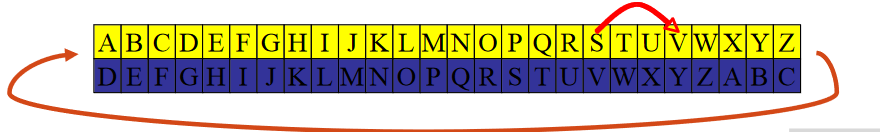
\includegraphics[width=0.9\textwidth]{03/cifrarioCesare.png}
                \caption{Esempio di cifrario di Cesare spostato di 3 posizioni}
            \end{figure}
        \subsubsection{Cifrario di Vigenère}
            Il \textbf{cifrario di Vigenère} è un cifrario che prevede l'uso di una "parola chiave", se necessario ripetuta per la lunghezza del messaggio, per poi calcolare la "somma" dei valori di ogni lettera del messaggio con la corrispondente lettera della parola chiave (prendendo poi il resto della divisione per 26). Quindi assegnando ad ogni lettera un numero da 0 a 25, si somma il numero della lettera del messaggio con il numero della lettera della parola chiave, si prende il resto della divisione per 26 e si assegna alla lettera corrispondente il numero ottenuto.
            \begin{figure}[H]
                \centering
                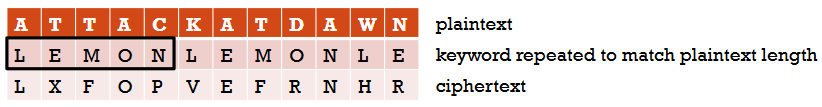
\includegraphics[width=0.9\textwidth]{03/cifrario2.png}
                \caption{Esempio di cifrario di Vigenère chiave "lemon"}
            \end{figure}
            Per decifrare il messaggio cifrato si sottrae il numero della lettera della parola chiave al numero della lettera del messaggio e si prende il resto della divisione per 26.
            \paragraph{Vantaggi} Questo cifrario è molto più sicuro rispetto a quello di cesare in quanto come mostrato nell'esempio la lettera "A" viene codificata in quattro lettere diverse e la lettera "T" che è presente tre volte viene cifrata in due lettere corrispondenti. In quanto la parola chiave ha lunghezza "l" allora dimensione della chiave è $l^{26}$. Inoltre se la chiave è della stessa lunghezza del messaggio allora il cifrario di Vigenère è equivalente a un cifrario di sostituzione casuale il che rende impossibile la decifrazione, però ciò comporta ad una ulteriore difficoltà per il mittente e il destinatario nel concordare una chiave.
    \subsection{Cifrari di trasposizione}
        \paragraph{In breve} I \textbf{cifrari di trasposizione} sono cifrari che permutano i simboli del messaggio in chiaro. In questo contesto la \textit{chiave} è la \textit{permutazione} dei simboli.
        \paragraph{In lungo} I \textbf{cifrari di trasposizione} sono dei \textbf{metodi di criptazione} per i quali i simboli del \textbf{messaggio in chiaro} sono permutati in un certo modo per ottenere il \textbf{messaggio cifrato}. Il ricevente decifra il testo svolgendo le permutazioni inverse.
        \subsubsection{Cifrario di trasposizione per colonne}
            Il \textbf{cifrario di trasposizione per colonne} è un cifrario che permuta i simboli del messaggio in chiaro per colonne, in modo che il messaggio cifrato sia una matrice di colonne.
            \begin{figure}[H]
                \centering
                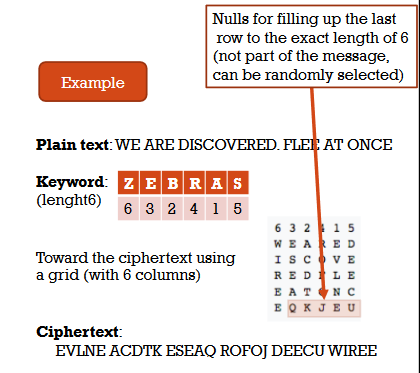
\includegraphics[width=0.5\textwidth]{03/cifrario3.png}
                \caption{Esempio di cifrario di trasposizione per colonne}
            \end{figure}
            Per decifrare il messaggio cifrato si riordinano le colonne in base alla chiave.
    \subsection{Criptografia Simmetrica}
        Come detto in precedenza la \textbf{criptografia simmetrica} prevede la stessa \textbf{chiave} per cifrare e de-cifrare i messaggi. La gestione di chi possiede le chiavi determina chi può accedere ai dati.
        \paragraph{Tipi} Esistono nella \textit{criptografia moderna} due tipi ci crittografia simmetrica:
        \begin{description}
            \item[Cifrari a flusso] I \textbf{cifrari a flusso} cifrano una "breve" porzione di un blocco di dati alla volta con una chiave che varia nel tempo. Questa tipologia si base su un \textbf{generatore di chiavi}, la cifratura è relativamente semplice (es. \texttt{XOR}) e molto spesso viene usato un bit per blocco.
            \item[Cifrari a blocchi] I \textbf{cifrari a blocchi} cifrano un blocco di dati "lungo" alla volta con una chiave fissa. Questa tipologia è più complessa e richiede uan funzione di cifratura e una di de-cifratura. Solitamente si usano blocchi di 64/128 bit.  
        \end{description}
        \subsubsection{Cifrari a flusso}
            I cifrari a flusso operano su un flusso di testo in chiaro e producono un flusso di testo cifrato. Lo stesso testo se ripetuto può essere cifrato in modo diverso in base al tempo nel quale è stato cifrato. I circuiti sono molto semplici e progettati per essere molto veloci.
            \begin{figure}[H]
                \centering
                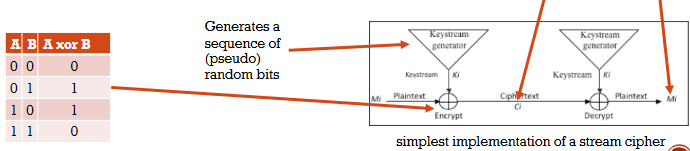
\includegraphics[width=0.9\textwidth]{03/cifrarioFlusso.png}
                \caption{Esempio di circuito di cifratura a flusso}
            \end{figure}
            \paragraph{Dove si usano} I cifrari a flusso sono usati in applicazioni in cui la velocità è fondamentale, come ad esempio nelle comunicazioni via radio o nella comunicazione in tempo reale.
        \subsubsection{Cifrari a blocchi}
    \chapter[\texttt{PKI} \& \texttt{TLS}]{Cryptography at work: \texttt{PKI} \& \texttt{TLS}}
\thispagestyle{chapterInit}
\section{Digital Certificates}
    \subsection{Introduzione}
        Il certificato digitale è un documento elettronico che contiene la chiave pubblica di un'entità, come un'organizzazione, un sito web o un individuo ben identificato tramite procedure di verifica dell'identità, spesso legislate da normative nazionali o internazionali. Il certificato è rilasciato da un'autorità di certificazione (CA) riconosciuta a livello internazionale, che garantisce l'identità del titolare del certificato. Il certificato è firmato digitalmente dalla CA, che ne garantisce l'integrità e l'autenticità. Il certificato può essere usato per autenticare l'identità del titolare, per garantire la riservatezza delle comunicazioni e per garantire l'integrità dei dati scambiati.
        Il certificato usa il paradigma della crittografia a chiave pubblica, in cui una chiave è usata per cifrare i dati e l'altra per decifrarli, infatti è composto da un certificato pubblico e da una chiave privata.
    \subsection{Struttura del certificato \texttt{X.509}}
        All'interno del certificato sono presenti le seguenti informazioni:
        \begin{description}
            \item[Version] o versione del certificato, che indica il formato del certificato.
            \item[Serial Number] o numero seriale del certificato, rispetto ad altri certificati rilasciati dalla stessa \texttt{CA}.
            \item[Signature Algorithm ID] o algoritmo di firma digitale usato per firmare il certificato.
            \item[Issuer] o autorità di certificazione, che ha rilasciato il certificato (\texttt{CA}).
            \item[Validity Period] o periodo di validità del certificato.
            \item[Subject] o titolare del certificato che lo ha richiesto, la quale identità è garantita dalla \texttt{CA}.
            \item[Subject Public Key] o chiave pubblica del titolare del certificato (\texttt{PK}).
                \subitem Algoritmo di cifratura asimmetrica usato per cifrare i dati.
                \subitem Valore della chiave pubblica.
            \item[Issuer Unique Identifier] o identificativo univoco della \texttt{CA}.
            \item[Subject Unique Identifier] o identificativo univoco del titolare del certificato.
            \item[Extensions] o estensioni del certificato, che possono contenere informazioni aggiuntive, quali nomi alternativi, restrizioni d'uso, ecc.
            \item[Signature] o firma digitale del certificato rilasciata dalla \texttt{CA} che garantisce l'integrità e l'autenticità del certificato e che questo non sia stato alterato o contraffatto.
        \end{description}
    \subsection{Certificati: domande e risposte}
        \begin{itemize}
            \item Come sono rilasciati i certificati?
            \item Chi può rilasciare i certificati?
            \item Perché dovrei fidarmi di un ente certificatore?
            \item Come posso controllare se un certificato è valido?
            \item Come posso revocare un certificato?
            \item Chi può revocare un certificato?
        \end{itemize}
        La risposta a queste domande è data dalla \texttt{PKI} (\texttt{Public Key Infrastructure}), che è un insieme di tecnologie, standard e procedure che permettono di gestire in modo sicuro le chiavi pubbliche e i certificati digitali.
\section{\textit{Public Key Infrastructure} - \texttt{PKI}}
    Una \texttt{PKI} è un insieme di tecnologie, standard e procedure che permettono di gestire in modo sicuro le chiavi pubbliche e i certificati digitali. Questa infrastruttura garantisce anche la corrispondenza tra le chiavi pubbliche e i titolari delle chiavi, garantendo l'integrità e l'autenticità delle chiavi pubbliche e dei certificati digitali.
    \subsection{Ottenere un certificato}
        Per ottenere un certificato, il titolare deve come prima cosa registrarsi presso una \texttt{CA} autorevole, la quale verifica tramite processi che possono essere automatici o manuali l'identità del richiedente. Una volta verificata l'identità del richiedente questo invia una chiave privata e pubblica da certificare alla \texttt{CA} la quale \texttt{CA} rilascia il certificato, contenete le informazioni del titolare e la chiave pubblica del titolare, questo certificato è firmato digitalmente tramite chiave privata dalla \texttt{CA} e inviato al titolare che ora può distribuirlo.
        \subsubsection{\texttt{ACME} - \texttt{Automated Certificate Management Environment}}
            \texttt{ACME} è un protocollo di gestione automatica dei certificati, che permette di automatizzare il processo di richiesta, rinnovo e revoca dei certificati digitali. Il protocollo è stato sviluppato per semplificare la gestione dei certificati digitali, riducendo i costi e i tempi di gestione dei certificati. Il protocollo è basato su un modello di autorizzazione a due fattori, in cui il richiedente deve dimostrare di avere il controllo del dominio per cui richiede il certificato e di essere autorizzato a richiedere il certificato.
            \paragraph{Let's encrypt} è un'autorità di certificazione che rilascia certificati digitali gratuitamente, tramite il protocollo \texttt{ACME}. Il servizio è stato lanciato nel 2016 con l'obiettivo di rendere l'uso dei certificati digitali più diffuso e sicuro, riducendo i costi e i tempi di gestione dei certificati. Il servizio è automatizzato e permette di ottenere un certificato digitale in pochi minuti, senza dover passare per procedure manuali di verifica dell'identità verificando l'identità del richiedente tramite il controllo del dominio per cui richiede il certificato.
            \paragraph{Funzionamento}\begin{enumerate}
                \item Il richiedente genere una coppia di chiavi pubblica e privata.
                \item Il richiedente dimostra di essere in possesso del dominio per cui richiede il certificato.
                \item Il richiedente richiede il certificato alla \texttt{CA} tramite il protocollo \texttt{ACME}.
                \item La \texttt{CA} verifica il controllo del dominio e rilascia il certificato.
                \item Il richiedente installa il certificato sul proprio server e può revocare o rinnovare il certificato in qualsiasi momento.
            \end{enumerate}
            \paragraph{Verifica del controllo del dominio}\begin{itemize}
                \item \texttt{HTTP-01}: il richiedente deve creare un file con un contenuto specifico e caricarlo sul proprio server web.
                \item \texttt{DNS-01}: il richiedente deve creare un record \texttt{TXT} con un contenuto specifico nel proprio server DNS.
                \item \texttt{TLS-ALPN-01}: il richiedente deve configurare un certificato particolare con una connessione \texttt{TLS} specifica.
            \end{itemize}
    \subsection{Requisiti su \texttt{PKI}}
        In quanto il sistema di \texttt{PKI} è distribuito a livello globale, è necessario che le \texttt{CA} e gli utenti rispettino alcuni requisiti comuni, tra cui: una politica di assegnazione nomi univoca, ogni parte della \texttt{PKI} deve provare ad alla \texttt{TTP} (\textit{Trusted Third Party}) che hanno una identità. Inoltre le \texttt{TTPs} devono controllare che quella identità sia valida e che il richiedente abbia ricevuto quella identità da una fonte affidabile. Infine le \texttt{TTPs} devono garantire che le chiavi pubbliche siano valide e che siano state rilasciate da una fonte affidabile.
        \paragraph{Requisiti dei software} Tutti i software che operano con la \texttt{PKI} devono rispettare alcuni requisiti, tra cui: devono supportare i protocolli standard della \texttt{PKI}, devono supportare i formati standard dei certificati digitali, devono supportare i meccanismi standard di verifica dei certificati digitali, devono supportare i meccanismi standard di revoca dei certificati digitali, devono supportare i meccanismi standard di gestione dei certificati digitali e devono essere aggiornati regolarmente per garantire la sicurezza dei certificati digitali.
        \subsubsection{\texttt{CRL} - \textit{Certificate Revocation List}}
            La \texttt{CRL} è una lista di certificati revocati, che contiene le informazioni sui certificati che sono stati revocati dalla \texttt{CA}. Questa lista viene aggiornata regolarmente dalla \texttt{CA} e distribuita in tutto il modo a orari regolari alle \texttt{RA} (\textit{Registration Authority}) e agli utenti. La \texttt{CRL} contiene le seguenti informazioni sui certificati revocati: il numero seriale del certificato, la data di revoca, il motivo della revoca e la \texttt{CA} che ha revocato il certificato. Una possibile criticità di questo sistema è che la \texttt{CRL} può essere ritardata nella sua distribuzione e quindi un certificato revocato può essere utilizzato per un certo periodo di tempo, non conosciuto per motivi di sicurezza.
    \subsection{Validazione di un certificato}
        La \textbf{validazione di un certificato} è il processo per il quale si verifica che un certificato sia valido, autentico e integro prima di stabilire una connessione \texttt{SSL/TLS} con un server web. Inoltre ci si assicura che il certificato non sia scaduto e che non sia stato revocato dalla \texttt{CA}. Il processo di validazione di un certificato è composto da diversi passaggi: \begin{enumerate}
            \item Il \textit{client} segue la catena di fiducia fino ad arrivare alla \texttt{CA} radice (\texttt{Root CA}).
            \item Ogni certificato nella catena di fiducia è verificato tramite la firma digitale della \texttt{CA} che lo ha rilasciato per garantire l'autenticità e l'integrità del certificato.
            \item Il \textit{client} verifica che il certificato sia valido per il periodo di validità specificato nei certificati.
            \item Viene controllato che il certificato non sia stato revocato dalla \texttt{CA} tramite la \texttt{CRL}.
            \item Infine il \textit{client} verifica che il \texttt{CN} (\textit{Common Name}) o il \texttt{SAN} (\textit{Subject Alternative Name}) del certificato corrisponda al nome del server web a cui si sta connettendo.
        \end{enumerate}
    \subsection{Catena di fiducia}
        La catena di fiducia è una struttura gerarchica che permette di garantire l'autenticità e l'integrità delle chiavi pubbliche e dei certificati digitali. La catena di fiducia è composta da una serie di entità che si fidano l'una dell'altra e che garantiscono l'autenticità e l'integrità delle chiavi pubbliche e dei certificati digitali. La catena di fiducia è basata su un modello gerarchico, in cui le entità sono organizzate in una struttura ad albero, in cui ogni entità è collegata a un'altra entità di livello superiore, fino ad arrivare a un'autorità di certificazione radice (\texttt{Root CA}).
\section{\texttt{SSL} \& \texttt{TLS} introduction}
    Come possiamo sfruttare la crittografia a chiave pubblica e l'infrastruttura \texttt{PKI} per garantire la riservatezza, l'integrità e l'autenticità delle comunicazioni su Internet? La risposta è data dal protocollo \texttt{SSL} (\textit{Secure Socket Layer}) e dal suo successore \texttt{TLS} (\textit{Transport Layer Security}), che permettono di garantire la sicurezza delle comunicazioni su Internet.
    \paragraph{\texttt{SSL}} (\textit{Secure Socket Layer}) è un protocollo di sicurezza che permette di garantire la riservatezza, l'integrità e l'autenticità delle comunicazioni su Internet. Il protocollo è basato su un modello di crittografia a chiave pubblica, in cui una chiave è usata per cifrare i dati e l'altra per decifrarli. Il protocollo è stato sviluppato da Netscape nel 1994 e ha avuto un grande successo, diventando uno standard de facto per la sicurezza delle comunicazioni su Internet.
    \paragraph{\texttt{TLS}} (\textit{Transport Layer Security}) è il successore di \texttt{SSL}, che è stato sviluppato per superare i problemi di sicurezza di \texttt{SSL} e per garantire una maggiore sicurezza delle comunicazioni su Internet. Il protocollo è basato su un modello di crittografia a chiave pubblica, in cui una chiave è usata per cifrare i dati e l'altra per decifrarli. Il protocollo è stato sviluppato dal gruppo di lavoro \texttt{IETF} (\textit{Internet Engineering Task Force}). Esistono varie versioni del protocollo, tra cui \texttt{TLS 1.0} (\texttt{RFC 2246} 1999), \texttt{TLS 1.1} (\texttt{RFC 4346} 2006), \texttt{TLS 1.2} (\texttt{RFC 5246} 2008), \texttt{TLS 1.3} (\texttt{RFC 8446} 2018), la versione \texttt{TLS 1.3} e \texttt{TLS 1.2} sono le più utilizzate e al momento coesistono nella rete.
    \paragraph{Obbiettivo di queste tecnologie} L'obiettivo di queste tecnologie è quello di garantire la riservatezza, l'integrità e l'autenticità delle comunicazioni nel web, proteggendo i dati sensibili degli utenti e garantendo la sicurezza delle transazioni online. Questo anche tramite il protocollo \texttt{HTTPS} (\textit{HyperText Transfer Protocol Secure}), che è una versione sicura del protocollo \texttt{HTTP} che utilizza il protocollo \texttt{SSL} o \texttt{TLS} per garantire la sicurezza delle comunicazioni tra il \textit{client} e il \textit{server} web.
    \chapter{Authentication II: \texttt{SSO}\& \texttt{SAML}}
\label{chap:authentication-ii}
\thispagestyle{chapterInit}
Questo capitolo è dedicato all'approfondimento dell'autenticazione all'interno di internet, in particolare verrà trattato il concetto di \texttt{Single Sign-On} per la riduzione del numero di credenziali da memorizzare e la gestione di queste ultime. Inoltre verrà trattato il protocollo \texttt{SAML} ovvero \textit{Security Assertion Markup Language} per la gestione di autenticazioni e autorizzazioni tra domini diversi, infine si parlerà di \texttt{SPID}, \texttt{CIE} \& \texttt{eIDAS} come esempi di implementazioni a livello nazionale ed europeo di \texttt{SSO}.
\section{Single Sign-On (\texttt{SSO})}
    \label{sec:sso}
    Il concetto alla base per il \texttt{SSO} è quello di avere un'unica autenticazione per accedere a (quasi) tutti i servizi, per raggiungere questo scopo il fornitore di servizi (\texttt{SP}) demanda il processo di autenticazione ad una autorità di identità (\texttt{IdP}) che si occupa di verificare che l'utente sia chi dice di essere, tramite i meccanismi visti precedentemente nella sezione \ref{sec:user-authentication}\footnote{\nameref{sec:user-authentication}}, mentre il processo di \textit{outsourcing} del processo di autenticazione è stato trattato nella sezione \ref{sec:outsourcing-authentication} \footnote{\nameref{sec:outsourcing-authentication}}.
    \paragraph{Funzionamento} Il funzionamento di un sistema \texttt{SSO} è il seguente:
        \begin{enumerate}
            \item L'utente accede all'applicazione \texttt{SP}
            \item L'applicazione \texttt{SP} reindirizza l'utente all'\texttt{IdP} per il processo di autenticazione
            \item L'\texttt{IdP} in primo luogo chiede all'utente di autenticarsi, il quale fornisce le proprie credenziali e l'\texttt{IdP} verifica l'identità dell'utente
            \item L'\texttt{IdP} genera un \textit{token} che viene cifrato e firmato con la chiave privata dell'\texttt{IdP} e inviato all'applicazione \texttt{SP}
            \item L'applicazione \texttt{SP} verifica la firma del \textit{token} con la chiave pubblica dell'\texttt{IdP} e se la verifica è positiva lo considera valido e lo inoltra all'utente che lo utilizzerà per accedere ai servizi (includendolo nelle richieste)
        \end{enumerate}
        Questo è il processo che avviene usualmente ma è possibile che il \textit{token} venga inviato all'utente dell'\texttt{IdP} e non direttamente all'applicazione del \texttt{SP}. In questo caso l'utente verifica la firma del \textit{token} con la chiave pubblica dell'\texttt{IdP} e poi lo includerà nelle richieste ai servizi.
    \paragraph{Proprietà} Le principali proprietà e vantaggi di un sistema \texttt{SSO} includono: la conservazioni delle credenziali in un unico posto e il non trasferimento delle stesse ad ogni servizio, i \textit{service provider} devono fidarsi dell'\textit{identity provider} nel verificare l'identità dell'utente. Inoltre il processo di autenticazione deve essere protetto, questo scopo lo si raggiunge usando la crittografia a chiave pubblica \footnote{ vedi \nameref{sec:PKI}} e con meccanismi di firma digitale.
    In questo paradigma è importante che l'\texttt{IdP} sia affidabile e che sia in grado di proteggere la \textit{confidentiality} e l'\textit{integrity} dei dati, inoltre è importante che l'\texttt{IdP} rimanga disponibile in quanto questo è un cosiddetto \textit{single point of failure}.
\section{Security Assertion Markup Language (\texttt{SAML})}
    \texttt{SAML} è un paradigma di autenticazione standard che sfrutta il formato \texttt{XML} per lo scambio di informazioni, questo lo rende molto \textit{verbose} anche per una piccola porzione di dati. Questo standard è stato introdotto nel 2002 e aggiornato nel 2005 in risposta alla mancanza di standard per lo scambio di informazioni di autenticazione e autorizzazione tra domini diversi.
    
    \begin{wrapfigure}{r}{0.25\textwidth}
        \centering
        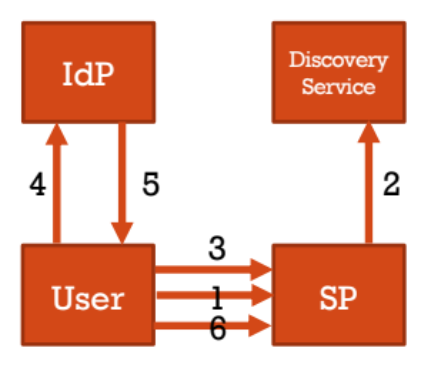
\includegraphics[width=0.25\textwidth]{05/SAML-Auth.png}
        \caption{Esempio di utilizzo di \texttt{SAML}}
    \end{wrapfigure}
    \paragraph{Esempio d'uso di \texttt{SAML}} In uno scenario dove ad esempio per avere uno sconto sul noleggio di un'auto è necessario essere membri VIP di una compagnia aerea, allora un utente (\textit{alice}) eseguirà il login sul sito della compagnia aerea (che agisce da \texttt{IdP} e \texttt{SP}) e poi verrà reindirizzata al sito di noleggio auto (che agisce solo da \texttt{SP}) con le informazioni dello status VIP dell'utente. A questo punto \textit{alice} può ottenere lo sconto da parte del sito di noleggio auto anche senza essersi autenticata su quest'ultimo, in quanto valgono le informazioni inviate dal sito della compagnia aerea.\newline
    In breve:
        \begin{enumerate}
            \item L'utente vuole accedere ad un servizio \texttt{SP}
            \item Questo servizio \texttt{SP} reindirizza l'utente ad un \textit{Discovery Service} che permettere all'utente di scegliere l'\texttt{IdP} per l'autenticazione
            \item Dopo essersi registrato tramite il \texttt{IdP} scelto l'utente torna al servizio \texttt{SP} con una identità valida verificato da un \texttt{IdP}
            \item Allora il fornitore di servizi rimanda l'utente al suo \texttt{IdP} per ottenere un \textit{token} di autorizzazione
            \item L'utente si autentica sul \texttt{IdP} e ottiene un \textit{token} di autorizzazione
            \item L'utente ritorna al servizio \texttt{SP} con il \textit{token} di autorizzazione e può accedere ai servizi
        \end{enumerate}
    
    \subsection{\texttt{SAML} Overview}
        Come mostrato in figura \ref{fig:saml-overview} l'architettura di \texttt{SAML} è composto da diversi componenti quali:
        \begin{description}
            \item[\textit{Assertions}] - Le dichiarazioni fatte dal \texttt{IdP} riguardo l'identità dell'utente
            \item[\textit{Protocols}] - I protocolli usati per lo scambio di informazioni tra i vari componenti
            \item[\textit{Bindings}] - I meccanismi usati per associare i protocolli di \texttt{SAML} con i protocolli di comunicazione
            \item[\textit{Profiles}] - La combinazione di \textit{Assertions}, \textit{Protocols} e \textit{Bindings} a supporto di uno specifico caso d'uso
            \item[\textit{Authentication Context}] - Un dettaglio sui tipo di autenticazione e livello di sicurezza
            \item[\textit{Metadata}] - Dati di configurazione per \texttt{IdP} e \texttt{SP}
        \end{description}
        \begin{figure}[H]
            \label{fig:saml-overview}
            \centering
            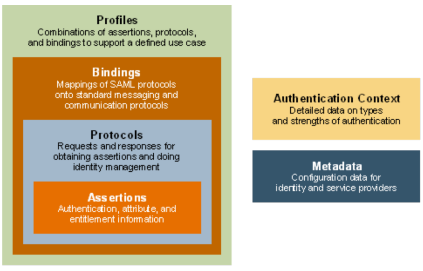
\includegraphics[width=0.5\textwidth]{05/SAML-Overview.png}
            \caption{Overview di \texttt{SAML}}
        \end{figure}
        \subsubsection{\textit{Assertions}}
            Le \textit{Assertions} sono le dichiarazioni fatte da una \texttt{SAML} \textit{authority} detta anche "parte dichiarante" (\textit{asserting party}). Le assertions possono essere viste come le unità di informazione di \texttt{SAML} e sono divise in tre tipi:
            \begin{description}
                \item[\textit{Authentication Assertion}] - Rilasciato dalla parte che autentica l'utente, contiene informazioni quali: chi ha autenticato l'utente, chi è il soggetto autenticato, quando è valida l'autenticazione, ecc\dots
                \item[\textit{Attribute Assertion}] - Contiene informazioni sullo stato dell'utente, come nell'esempio di \textit{alice} l'appartenenza al programma VIP
                \item[\textit{Authorization Assertion}] - Contiene informazioni su cosa può fare l'utente, come ad esempio la possibilità di noleggiare un'auto quando in viaggio di lavoro
            \end{description}
            \paragraph{\textit{Authentication Assertion}}
                Questo tipo di \textit{assertion} è strutturato nel seguente modo:
                \begin{description}
                    \item[Intestazione] - Contiene informazioni sulla versione di \texttt{SAML} usata, lo schema per \texttt{XML} e l'ora di creazione (\textit{issue instant})
                    \item[Autorità] - Contiene informazioni sul \texttt{IdP} che ha rilasciato l'\textit{assertion}
                    \item[Soggetto] - Contiene un identificativo univoco che rappresenta l'utente autenticato
                    \item[Condizioni] - Contiene informazioni sulla validità dell'\textit{assertion} (vale non prima di, non dopo il) con data e ora
                    \item[\textit{Authenticating Context}] - Contiene informazioni sul tipo di autenticazione e il livello di sicurezza che è stato usato\footnote{Si noti come la autenticazione in se non è parte del \texttt{SAML}, nelle \textit{assertion} ci si riferisce ad un processo di autenticazione avvenuto precedentemente}
                \end{description}
            \paragraph{\textit{Attribute Assertion}}
                Questo tipo di \textit{assertion} è strutturato nel seguente modo:
                \begin{description}
                    \item[Intestazione] - Contiene informazioni sulla versione di \texttt{SAML} usata, lo schema per \texttt{XML} e l'ora di creazione (\textit{issue instant}) l'unica differenza con l'\textit{Authentication Assertion} è il tipo di schema usato
                    \item[Attributo] - Contiene un identificatore del tipo di attributo (solitamente in modo molto specifico) e il valore dell'attributo
                \end{description}
        \subsubsection{\textit{Protocols}}
            I protocolli sono i meccanismi usati per lo scambio di asserzioni tra le varie parti e descrivono come poterne ottenerne una, come usarla e come verificarla. Vengono definiti anche protocolli sulle richieste di autenticazione e sulla risoluzione di parametri "passati per riferimento", viene definito anche un protocollo per il \textit{single logout} e per la gestione delle sessioni, e molo altro\dots\newline
            Distinguiamo come protocolli di comunicazione quei sistemi che permettono a due o più entità di scambiarsi informazioni definendo regole, semantica, sintassi e sincronizzazione. Esistono inoltre i protocolli di criptografia che sono designati alla protezione della comunicazione tra due entità, vengono applicati usando i \textit{cryptographic primitives} (come funzioni di \textit{hash}, cifrature simmetriche e asimmetriche, ecc\dots).
        \subsubsection{\textit{Bindings}}
            I \textit{bindings}, come anticipato, sono i meccanismi usati per definire i meccanismi per il trasporto dei messaggi \texttt{SAML} su protocolli di comunicazione diversi, come ad esempio \texttt{SAML URI}, \texttt{SAML SOAP}, \texttt{HTTP Redirect}, \texttt{HTTP POST}, ecc\dots
            \paragraph{\texttt{HTTP Redirect}} Questo meccanismo, in particolare, permette la trasmissioni di messaggi \texttt{SAML} tramite parametri di \texttt{URL} in una richiesta. In questo modo viene usato lo \textit{UserAgent} come intermediario per la trasmissione dei messaggi, questo meccanismo potrebbe essere necessario se è richiesta l'interazione con l'utente per generare una risposta. Questo è di gran lunga il meccanismo più usato (oltre che il preferito) per la trasmissione di messaggi \texttt{SAML} e per il \texttt{SSO}.
        \subsubsection{\textit{Profiles}}
            I \textit{profiles} sono le specifiche che definiscono come usare le \textit{assertions}, i \textit{protocols} e i \textit{bindings} per supportare uno specifico caso d'uso. Questi profili sono definiti per specifici scenari di utilizzo e sono usati per definire le regole di interazione tra le varie parti. I profili sono definiti per specifici scenari di utilizzo e sono usati per definire le regole di interazione tra le varie parti. 
            \paragraph{\textit{Web browser \texttt{SSO}}} Il profilo più comune è il \textit{web browser \texttt{SSO}} il quale ha più opzioni per quello che riguarda l'inizio e il trasporto dei messaggi \texttt{SAML}. L'inizio del flusso dei messaggio può essere inizializzato dal \texttt{SP} o dal \texttt{IdP} e il trasporto dei messaggi può essere eseguito tramite diversi \textit{bindings} quali \texttt{HTTP Redirect}, \texttt{HTTP POST}, \texttt{HTTP Artifact}, ecc\dots
            \paragraph{\textit{Single Logout}} Questo profilo è usato per terminare tutte le sessioni attive di un utente in una specifica rete \texttt{SAML}. In questo profilo l'utente ha stabilito un precedenza più sessioni con più \texttt{SP} ed un \texttt{IdP} e vuole terminare tutte le sessioni attive. Le sessioni gestite da una \textit{Session Authority} (\texttt{SeA}) che è un'entità che mantiene le informazioni sulle sessioni attive e che permette di terminarle (molto spesso è l'\texttt{IdP}). Quando l'utente vuole terminare la sessione, invia una richiesta di \textit{logout} alla \texttt{SeA} che termina tutte le sessioni attive inviando un messaggio di \textit{logout} a tutti i \texttt{SP} e all'\texttt{IdP}.
        \subsubsection{\textit{Authentication Context}}
            Questo componente indica come un utente si è autenticato presso un \texttt{IdP}. È quindi compito dell'\texttt{IdP} includerlo nelle \textit{assertions} in base alle richieste del \texttt{SP} o in base alla configurazione dell \texttt{IdP}. Le informazioni dentro l'\textit{authentication context} vengono usate per determinare il "livello di assicurazione" dell'autenticazione, ovvero quanto si è certi che l'utente sia chi dice di essere e di conseguenza quante e quali risorse può accedere. Solitamente un \textit{Level Of Assurance} (\texttt{LoA}) è costituito da un numero e definito in base al "valore" del "rischio" che è necessario per l'accesso alle risorse, questi livelli si basano principalmente su nozioni base di autenticazione.
        \subsubsection{\textit{Metadata}}
            Questo componente è usato per definire i dati di configurazione per \texttt{IdP} e \texttt{SP} e contiene informazioni quali: qual è l'identificativo dell'entità, le chiavi di criptografia, gli \textit{endpoints} per la comunicazione, ecc\dots Ogni entità di un sistema \texttt{SAML} ha un \textit{entity ID} che la identifica univocamente all'interno del sistema. Questo viene usato per associare le chiavi pubbliche alle entità e quindi per verificare le firme digitali. In entrambi le situazione gli \textit{id} e le chiavi pubbliche devono essere scambiate precedentemente in modo sicuro.
        
            
        \subsubsection{Correlazione tra le componenti}
            Le componenti di \texttt{SAML} sono correlate tra loro in questo modo: b
            \begin{description}
                \item[\textit{Assertions \& Protocols}] - Corrispondono al livello di applicazione del modello \texttt{ISO/OSI}. Da questo livello abbiamo la \textit{SSO experience}.
                \item[\textit{Bindings}] - Sono posizionati tra il livello dei profile e il livello applicazione.
                \item[\textit{Profiles}] - Sono posizionati al sotto il livello di applicazione e comunicano con questo tramite i \textit{bindings}.
            \end{description}
            I \textit{profiles} insieme ai \textit{bindings} costituiscono il \textit{web-service} dove sono specificate le tecnologie da usare quali \texttt{XML}, \texttt{URL}, \texttt{HTTP}, \texttt{HTTPS}, \texttt{SOAP}, ecc\dots
    \subsection{La sicurezza di \texttt{SAML}}
        La sicurezza di \texttt{SAML} non è propriamente intrinseca al protocollo, in quanto un semplice attacco del tipo \textit{men-in-the-middle} potrebbe ottenere la \textit{assertion} e usarla più tardi sostituendosi all'utente. Per questo motivo il protocollo \texttt{SAML} definisce, oltre ai meccanismi di scambio di informazioni, anche i meccanismi di protezione delle informazioni scambiate, principalmente viene usata la \texttt{PKI}\footnote{Vedi \ref{sec:PKI} \nameref{sec:PKI}} la quale però non è obbligatoria, ma è fortemente raccomandata.
        \paragraph{Qualche possibile attacco} Alcune possibili vulnerabilità di \texttt{SAML} riguardano: il tempo di validità di un \textit{assertion}, risolvibile inserendo una durata relativamente breve, la ripetizione di un \textit{assertion}, risolvibile inserendo accettando solo una volta un \textit{assertion} con uno stesso \texttt{ID}, la ricezione di un \textit{assertion} per un \textit{SP} diverso, tutti i \textit{SP} devono accettare solo ed esclusivamente i messaggi destinati a loro e non a un altro \textit{SP}. Inoltre esiste una possibile vulnerabilità relativa a \texttt{XXE} o \textit{XML External Entity}, il quale sfrutta il fatto che \texttt{SAML} è basato su \texttt{XML} inviati dall'utente e poi processati dal \texttt{SP}, ma in quanto \texttt{XML} è molto pesante da processare ciò potrebbe portare ad un \textit{DoS} o ad un \textit{XXE}.

        \paragraph{Privacy e \texttt{SAML}} La privacy è un aspetto molto importante per \texttt{SAML} in quanto le informazioni scambiate sono molto sensibili, allora è possibile non scambiare direttamente le informazioni ma passare solo un codice identificativo dell'entità che possa essere usato per recuperare le informazioni dal \texttt{IdP}. Il problema però rimane che se l'\texttt{IdP} è compromesso o "venduto" allora tutte le informazioni, sia quelle di tipo identificativo che quelle associate ad un "\textit{log}" dei servizi a cui si è acceduto, sono a rischio.
\section{Infrastruttura di identità nazionale}
    \subsection{SPID - Sistema Pubblico di Identità Digitale}
        \paragraph{Struttura generale} Lo \texttt{SPID} è un sistema di identità digitale che permette di accedere a tutti i servizi online della pubblica amministrazione e di altri enti privati con un'unica identità digitale. Questo sistema si basa su \texttt{SAML 2.0} ma esistono due entità in più, la prima è "\texttt{AgID}" che ha il compito di coordinare e gestire il sistema fornendo ai \texttt{SP} l'elenco degli \texttt{IdP} autorizzati e la seconda è \textit{Attribute Provider} che fornisce informazioni aggiuntive sull'utente. A linee generali il funzionamento è lo stesso di \texttt{SAML} con l'aggiunta di un "passo 0" che consiste nel \texttt{SP} che chiede ad \texttt{AgID} l'elenco degli \texttt{IdP} autorizzati e un passaggio opzionale per il \texttt{SP} che chiede all'\textit{Attribute Provider} informazioni aggiuntive sull'utente.
        \paragraph{La legge} A livello legale per diventare \texttt{IdP} o \texttt{SP} bisogna rispettare delle norme sia a livello italiano che a livello europeo, queste norme si pongono al di sopra dello standard \texttt{SAML} e all'infrastruttura tecnica, queste sono state introdotte per aumentare il livello di sicurezza e di privacy delle informazioni scambiate, inoltre prevedono che se necessario a livello giudiziario si possano ottenere (parte) delle informazioni scambiate. 
    \chapter{Access Control I}
\label{chap:accessControl}
\thispagestyle{chapterInit}

\paragraph{Obbiettivi} Gli obbiettivi dei sistemi di controllo degli accessi sono:
    \begin{itemize}
        \item \textbf{Confidenzialità}: garantire che le informazioni siano accessibili solo a chi è autorizzato.
        \item \textbf{Integrità}: garantire che le informazioni non siano alterate da chi non è autorizzato.
    \end{itemize}

\section{\textit{Access Control}}
    \begin{figure}[H]
        \label{fig:accessControlSchema}
        \centering
        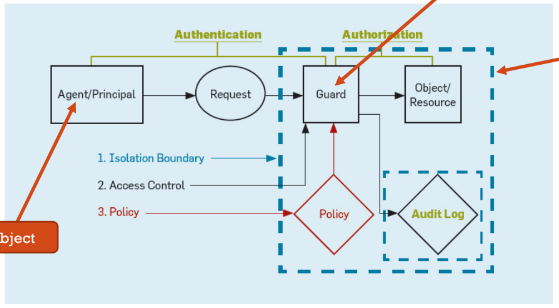
\includegraphics[scale=0.5]{06/AccessControSchema.png}
        \caption{Schema di un sistema di controllo degli accessi}
    \end{figure}

    Dallo schema raffigurato possiamo denotare che:
    \begin{itemize}
        \item \textbf{Soggetto} (\textit{Agent/Principal}): è l'entità che vuole accedere ad un oggetto o una risorsa, questo deve essere autenticato e autorizzato per poter accedere. Ad esempio un operatore di cassa di una banca non può accedere ai dati dei clienti, ma dopo aver ricevuto opportuna autorizzazione può effettuare operazioni sui conti.
        \item \textbf{Richiesta} (\textit{Request}): è la richiesta di accesso fatta dal soggetto. Questa contiene diverse informazioni che vedremo in seguito.
        \item \textbf{Confine di Isolamento} (\textit{Isolation Boundary}): è il confine che separa il soggetto dal sistema che contiene l'oggetto o la risorsa. Questo confine è importante per garantire che il soggetto non possa accedere direttamente all'oggetto o alla risorsa.
        \item \textit\textbf{Guard} (\textit{Policy Decision Point}): è l'entità che decide se il soggetto può accedere all'oggetto o alla risorsa. Questo prende decisioni basandosi su regole di autorizzazione.  
        \item \textit\textbf{Policy}: è l'insieme di regole che il \textit{guard} deve seguire per decidere se il soggetto può accedere all'oggetto o alla risorsa.
        \item \textbf{Oggetto} (\textit{Object/Resource}): è l'entità a cui il soggetto vuole accedere. Questo può essere un file, un database, un dispositivo, ecc\dots Questo deve essere protetto per garantire la confidenzialità e l'integrità delle informazioni.
        \item \textbf{Sistema Controllo Accessi} (\textit{Access Control }): è il punto dove avviene il controllo degli accessi. (Solitamente il \textit{guard} è una parte di questo sistema).
        \item \textit\textbf{Audit Log}: è il registro che contiene tutte le informazioni riguardanti le richieste di accesso sia autorizzate che non autorizzate. Questo è importante per monitorare il sistema e per rilevare eventuali attacchi.
    \end{itemize}
    
    \paragraph{Alcune note} Il confine di Isolamento tra il soggetto e tutto il resto del sistema è molto importante per garantire che nessuno possa accedere direttamente all'oggetto o alla risorsa senza passare per il \textit{guard}. Solo degli utenti con privilegi speciali, quali "amministratori" possono \textit{by-passare il guard} questo solo per aggiornare delle \textit{policy} o altri aggiornamenti al sistema. Infine è presente anche una \textit{inner boundary} che garantisce l'integrità dell'\textit{audit log}, questa non può essere \textit{by-passata} da nessuno, nemmeno dagli amministratori.
    \subsection{I Sistemi Operativi}
        I sistemi operativi sono esempi di sistemi che implementano il controllo degli accessi. Questi infatti non permettono di accedere direttamente alle risorse \textit{hardware} e \textit{software} del sistema, ma forniscono un'interfaccia per accedere a queste. Inoltre alcuni \texttt{SO} supportano multi-utente e multi-tasking, dove per il primo bisogna implementare un sistema per garantire accesso allo stesso tempo e/o in modo concorrente a più utenti, mentre per il secondo bisogna sviluppare un sistema per garantire che più processi in parallelo possano accedere alle risorse del sistema in modo concorrente.
        \subsubsection{Struttura del \texttt{SO}}
            Un sistema operativo è composto da una memoria, accessibile agli utenti, la quale comunica con il sistema operativo che tramite appositi meccanismi di controllo degli accessi permette di accedere al \texttt{I/O} \textit{bus} dove sono collocate le \texttt{I/O} \textit{interfaces} che permettono di accedere alle risorse del sistema (dischi, stampanti,\dots).\newline
            In questo sistema bisogna proteggere la memoria, i file contenuti nei dischi, controllare l'accesso degli utenti tramite meccanismi di autenticazione e autorizzazione e infine proteggere in generale il controllo degli accessi.
            \paragraph{Cosa implementa \texttt{SO}} Facendo riferimento alla figura \figref{fig:accessControlSchema}, il sistema operativo dunque implementa l'autenticazione, l'autorizzazione e la barriera di isolamento esterna per garantire che le \textit{policy} siano rispettate.
    \subsection{Definizione, Scopo e \textit{Policy} di un \texttt{AC}}
        \paragraph{Definizione} Un sistema di controllo accessi è definito come il processo che \textbf{media} le \textbf{richieste} alle risorse e ai dati di un sistema determinando se la richiesta di accesso deve essere approvata o rifiutata.
            \subparagraph{\textit{Flow} della richiesta} \begin{enumerate}
                \item Una richiesta di accesso $(s,a,r)$ viene fatta da un soggetto $s$ per accedere ad un oggetto $r$ tramite un'azione $a$. Questa arriva al modulo di controllo accessi
                \item Il modulo di controllo accessi prende la decisione se approvare (\textit{grant}) o rifiutare (\textit{deny}) la richiesta.
                \item Se la risposta è \textit{grant} allora $s$ può eseguire l'operazione $a$ su $r$, altrimenti se la risposta è \textit{deny} allora $s$ è informato che \underline{non} può eseguire l'operazione $a$ su $r$.
            \end{enumerate}
        Questo processo è di fondamentale importanza in un qualsiasi sistema di sicurezza.
    \subsection{Struttura di un \texttt{AC}}
        \paragraph{\textit{Policy}} La \textit{policy} sono le regole, ad alto livello, che controllano chi può accedere e che azioni possono eseguire su una particolare risorsa, o oggetto, che contiene informazioni.
        \paragraph{\textit{Model}} Il \textit{model} è la rappresentazione matematica formale della \textit{policy}, e come funziona una \textit{policy} in un sistema di controllo accessi.
        \paragraph{\textit{Enforcement}} L'\textit{enforcement} è l'\textit{hardware} o il \textit{software} che, a basso livello, implementano i controlli imposti dalle \textit{policy} e formalmente descritti nel \textit{model}.
        % Durante il corso è stato tralasciato la sezione "What can go wrong" 
\section{\textit{Access Control Models}}
    Il significato delle \textit{policy} si basa nella forma:
    \begin{quote}
        "Un soggetto $s$ può eseguire un'azione $x$ su un oggetto $o$
    \end{quote}
    una serie di queste affermazioni possono essere espresse nella forma di una matrice di controllo degli accessi (\textit{Access Control Matrix} \texttt{ACM}). Questa matrice è composta da righe e colonne, dove le righe rappresentano i soggetti (utenti) e le colonne rappresentano gli oggetti (risorse/files) e le celle contengono informazioni su chi è il proprietario dell'oggetto, chi può leggere o scrivere su di esso, ecc\dots
    \begin{table}[H]
        \centering
        \begin{tabular}{c|c|c|c|c|c|c|}
            \multicolumn{1}{c}{} & \multicolumn{1}{c}{\textit{f1}} & \multicolumn{1}{c}{\textit{f2}} & \multicolumn{1}{c}{\textit{f3}} & \multicolumn{1}{c}{\textit{f4}} & \multicolumn{1}{c}{\textit{f5}} & \multicolumn{1}{c}{\textit{f6}} \\
            \cline{2-7}
            \textit{s1} & &\textit{o, r, w} & \textit{o, r, w} &&& \\
            \cline{2-7}
            \textit{s2} & \textit{o, r, w} & \textit{r} & & & \textit{o, r, w} & \\
            \cline{2-7}
            \textit{s3} & & \textit{r} & \textit{r} & \textit{o, r, w} & \textit{r} & \textit{o, r, w} \\
            \cline{2-7}
        \end{tabular}
        \caption{Esempio di una \textit{Access Control Matrix}}
    \end{table}
    Altri sistemi di controllo accessi sono:
    \begin{itemize}
        \item \textit\textbf{Capability} (\texttt{C-list}): è un sistema dove ogni soggetto possiede una lista di capacità che gli permettono di accedere a determinate risorse. 
        \item \textit\textbf{Accesso Control List} (\texttt{ACL}): è un sistema dove ogni oggetto ha una lista di controllo degli accessi che contiene i soggetti che possono accedere all'oggetto e le azioni che possono eseguire.
    \end{itemize}
    Entrambe queste sono migliori della \texttt{ACM} in termini di efficienza, dato che non occupiamo spazio per le celle vuote ed sono molto più scalabili, il problema di tutte e tre è che bisogna verificare a monte se il richiedente è veramente chi dice di essere.

    \subsection{\texttt{ACL} v/s \texttt{C-list}}
        In questo genere di sistemi si usa come meccanismo di interazione con il sistema un \textit{compiler service} il quale si non può direttamente accedere e/o scrivere su un file, ma grazie ai permessi che eredita dagli utenti può farlo. Mentre il processi di lettura/scrittura avvengono viene aggiunta una riga ad un \textit{Bill file} il quale non può mai essere modificato direttamente da nessuno, ma solo dal \textit{compiler service} il quale vi scrive le informazioni necessarie per il controllo degli accessi.\newline
        Può accadere che il \textit{caller} confonda il \textit{compiler service} il quale restituisce il nome del \textit{billing file} al posto dell'oggetto richiesto in output, in questo caso l'integrità dell'\textit{Bill file} è compromessa e il sistema non è più sicuro.
        \subsubsection{\texttt{ACL}}
            Nel caso si usi un sistema \texttt{ACL} il problema risiede nel fatto che durante le operazioni il \textit{compiler service} è delegato dall'utente per l'accesso al file di output, e dal \texttt{SO} per l'accesso al \textit{billing file}. In quanto l'accesso avviene nella stesse esecuzione il \textit{compiler service} non può distinguere se l'accesso è stato fatto per conto dell'utente o del \texttt{SO}, quindi l'utente può scrivere sul \textit{billing file} e compromettere l'integrità del sistema.
        \subsubsection{\texttt{C-list}}
            Nel caso si usi un sistema \texttt{C-list} questo problema non si presenta in quanto l'utente non deve delegare esplicitamente l'accesso al file di input al \textit{compiler service} in quanto è il \texttt{SO} a farlo, quindi i permessi non vengono mai delegati dall'utente al \textit{compiler service}, ciò permette di evitare di confondere il \texttt{SO} con l'utente quando si scrive sul \textit{billing file}.
    \subsection{\textit{Confused Deputy in the cloud}}
        Il problema appena descritto si applica anche nel \textit{cloud}. Ad esempio se in un servizio si vuole delegare l'accesso a file o risorse ad altri account, questo è un esempio di accesso delegato. Nel cloud il problema di "\textit{confused deputy}" può accedere quando due utenti \texttt{A} e \texttt{B} ottengono il diritto all'esecuzione di un servizio \texttt{M}: Nel momento nel quale \texttt{A} viene concesso il diritto di scrittura viene inserita la coppia $(r,\texttt{M})$ nella \texttt{ACL} del servizio, quando ora \texttt{B} chiede di eseguire il servizio \texttt{M} per monitorare le risorse di \texttt{A} dato che \texttt{B} ha il diritto di eseguire il servizio \texttt{M} può leggere anche le risorse di \texttt{A}.\newline
        Per prevenire ciò bisogna implementare un \textbf{identificatore esterno} che deve essere univoco per ogni istanza del servizio \texttt{M}
    \subsection{Digressione sulla protezione nei sistemi operativi}
        Gli obbiettivi del \texttt{AC} per la protezione nei sistemi operativi sono:
        \begin{itemize}
            \item La prevenzione di uso malizioso delle risorse da parte degli utenti e/o processi.
            \item Il controllo che le risorse condivise siano usate secondo le \textit{policy} stabilite.
        \end{itemize}
        Per garantire ciò vengono stabiliti dei principi di protezione quali:
        \begin{description}
            \item[Principio del minimo privilegio] Un utente/processo deve avere solo i privilegi necessari per eseguire il suo compito. Questo garantisce che se un utente/processo è compromesso, il danno che può fare è limitato al suo ambiente e non può compromettere l'intero sistema.
            \item[Principio della conoscenza minimale] Un utente/processo deve avere accesso solo agli oggetti che deve conoscere per eseguire il suo compito. In questo modo si evita che un utente/processo possa accedere a risorse che non dovrebbe conoscere.
            \item[Dominio di protezione] Un dominio di protezione è una serie di oggetti e permessi che un utente/processo può eseguire su quegli oggetti. Formalmente un dominio di protezione è definito come segue: $$ \left< \texttt{object}, \{ \texttt{access rights} \} \right>$$ I domini di protezione possono essere implementati per utenti, processi o procedure. Un esempio di dominio di protezione è negli ambienti Unix/Linux dove ogni utente corrisponde ad un dominio di protezione.
        \end{description}
    \subsection{\texttt{AC} \textit{Models}}
        Esistono molti modelli di controllo degli accessi, i principali sono però:
        \begin{itemize}
            \item \texttt{DAC} (\textit{Discretionary Access Control}) I soggetti possono dare autorizzazione ad altri soggetti (\texttt{DISCRETIONARY})
            \item \texttt{MAC} (\textit{Mandatory Access Control}) Il sistema forza le regole di accesso (\texttt{MANDATORY})
        \end{itemize}
        \paragraph{\texttt{DAC}} I vantaggi in un modello \texttt{DAC} consistono principalmente nella flessibilità rispetto ad ogni singolo utente, inoltre la possibilità di delegare l'autorizzazione ad altri utenti rende questo sistema molto discrezionale, infatti il principale svantaggio è la difficoltà di gestire le autorizzazioni in un sistema con molti utenti da parte di un organo centrale, ciò significa che se ad esempio un utente non-it si dimentica di rimuovere un utente da una lista di controllo degli accessi, questo potrebbe avere accesso a risorse che non dovrebbe avere. Inoltre, se un utente è compromesso, allora tutte le risorse a cui ha accesso sono compromesse.
            \subparagraph{\texttt{DAC} \& gruppi} Nelle grandi organizzazioni è molto comune usare i gruppi per gestire le autorizzazioni, in quanto è molto più facile gestire i permessi di un gruppo piuttosto che di un singolo utente.
            \subparagraph{Attacchi \textit{trojan}} Un problema al quale i sistemi \texttt{DAC} sono soggetti è l'attacco \textit{trojan}, dove un utente malintenzionato (\textit{bob}) che normalmente non può accedere ad una risorsa ($r$) creando una risorsa $r'$ a cui può accedere e convincendo \textit{alice}, un utente autorizzato ad accedere alla risorsa originale $r$, a installare un programma \textit{trojan}, tramite tecniche di \textit{social engineering}, il quale legge il contenuto di $r$ e lo scrive su $r'$, in questo modo \textit{bob} può accedere alle informazioni di $r$.
        \paragraph{\texttt{MAC}} I vantaggi di un modello \texttt{MAC} sono che il sistema forza le regole di accesso, quindi non c'è bisogno di fidarsi degli utenti in quanto questi sono verificati e autorizzati da un organo centrale. Inoltre, se un utente è compromesso, solo le risorse a cui ha accesso sono compromesse, le altre risorse sono al sicuro. Gli svantaggi sono che il sistema è molto rigido e non flessibile, quindi per cambiare le autorizzazioni bisogna passare per un organo centrale, inoltre è molto difficile da implementare in sistemi con molti utenti.
            \subparagraph{Esempi di \textit{policy}} I permessi degli utenti vengono decisi dall'organizzazione che provvede anche a regolare come le risorse devono essere condivise. Ad esempio in un ospedale i dati dei pazienti non possono essere condivisi ed solo i medici che curano il paziente possono accedere ai dati del paziente. Viene introdotta anche una \textit{security label} che indica il livello di sicurezza, il personale che vi può accedere e l'orario di creazione della risorsa.
    \subsection{Sicurezza multi-livello}
        Le prime necessità nel garantire la sicurezza si sono verificate nel campo militare, dove diversi gradi di utenti possono accedere a diverse risorse, basate sul loro grado. Questo problema è nato ancora prima dell'avvento dei computer. Per garantire l'accesso a diversi livelli di risorse vengono effettuati dei controlli di sicurezza per evitare che utenti non autorizzati possano diffondere informazioni sensibili.
        \subsubsection{Implementazione}
            Per categorizzare le informazioni vengono introdotti dei livelli di \textit{sensitivity} in base a quanto quella risorsa è sensibile. Questi livelli vengono poi associati ad ogni risorsa in modo lineare all'importanza della risorsa. Esistono i livelli \textit{Top Secret} $\geq$ \textit{Secret} $\geq$ \textit{Confidential} $\geq$ \textit{Unclassified}. Questi livelli vengono poi associati ad ogni utente in base al loro grado, in modo che un utente con un grado più basso non possa accedere a risorse con un livello di sensibilità più alto.
        \subsubsection{Associazione dei livelli}
            Quando si crea una risorsa vi è associato il livello di \textit{sensitivity} e la corrispondente \textit{security label}, ciò avviene in base a criteri definiti in precedenza. Se in un documento sono presenti informazioni di livelli diversi allora il livello di sensibilità del documento sarà il livello più alto tra quelli presenti nel documento.\newline
            Esiste inoltre la possibilità che dopo qualche tempo il livello di sensibilità di una risorsa possa cambiare, in questo caso bisogna aggiornare la \textit{security label} della risorsa con il nuovo livello di sensibilità.
            \paragraph{Associazione agli utenti}
                Una volta che una risorsa è stata associata ad un livello di sensibilità, bisogna stabilire quali utenti sono autorizzati ad accedere a quella risorsa. Questo viene fatto associando ad ogni utente un livello di autorizzazione, che ha la stessa struttura di un livello di sensibilità. Un utente può accedere ad una risorsa se il suo livello di autorizzazione è maggiore o uguale al livello di sensibilità della risorsa. Formalmente una "\textit{clearance}" $C$ è composta da un livello di sicurezza gerarchico $S$ che indica il grado di affidabilità dell'utente ed un insieme di risorse "\textit{need-to-know}" $N$ che indica le risorse a cui l'utente deve poter accedere. ($C = (S,N)$)
        \subsubsection{Proprietà}
            Le proprietà di un sistema multi-livello sono:
            \begin{itemize}
                \item \textit\textbf{No read Up}: Un utente $s$ può leggere una risorsa $r$ se e solo se $(Ss,Ns)$ \textbf{domina} $(Sr,Nr)$ 
                \item \textit\textbf{No write Down}: Un utente $s$ può scrivere su una risorsa $r$ se e solo se $(Sr,Nr)$ \textbf{domina} $(Ss,Ns)$
            \end{itemize}
            Per \textbf{domina} intendiamo che $(S1,N1)$ domina $(S2,N2)$ se $S1 \geq S2$ e $N1 \supseteq N2$.\newline
            Anche se può sembrare contro-intuitivo il fatto che un utente con un livello di sensibilità più bassa possa scrivere su una risorsa con un livello di sensibilità più alto, questo è necessario non per garantire l'integrità della risorsa, ma per garantire la confidenzialità delle informazioni.
            % Multi-Level Security (6,7) SKIP
        \subsubsection{Pro e contro}
            I vantaggi di un sistema multi-livello sono che il sistema non è soggetto ad attacchi \textit{trojan} per la proprietà di \textit{no write down}, inoltre è rigido il che permette di tenere la situazione di controllo accessi sotto controllo, d'altra parte per cambiare le autorizzazioni bisogna passare per un organo centrale, inoltre il sistema è soggetto a \textit{information leakage by covert channels}, ovvero il passaggio di informazioni per mezzo di canali che nin sono stati progettati per trasmettere informazioni (eg. si è riuscito ad ottenere informazioni su quello che viene detto in una stanza analizzando il livello di luminosità della lampadina).
    \subsection{Ruolo / Gruppo / Utenti / Soggetti / Permessi / Sessioni - Definizioni}
        \subsubsection{Ruoli e Gruppi}
            Anche se i concetti di ruolo e gruppo possono sembrare simili, in realtà nella loro applicazione assumono un significato diverso. Formalmente:
            \begin{quote}
                Un \textit{ruolo} è un tipo di lavoro nel contesto di un'organizzazione, con della semantica associata, questa relativa le autorità e le responsibilità conferite al soggetto il quale ricopre quel ruolo.\texttt{[ANSI RBAC Standard]}
            \end{quote}
            Dunque i ruoli permettono di gestire i premessi in modo indiretto rispetto agli utenti, si può associare uno o più ruoli ad un utente e poi associare i permessi per eseguire una certa operazione a quel ruolo.\newline
            Un gruppo, molto più semplicemente, è un insieme di utenti.\newline
            Questo significa che ad un gruppo può essere associato un ruolo, ma ad un gruppo non può essere associato un permesso, questo in quanto i permessi non sono una cosa propria di un gruppo, ma di un ruolo.
        \subsubsection{Utenti e Soggetti}
            Spesso utente e soggetto vengono usati come sinonimi, nel nostro caso possiamo usarli come tali definendo:\newline
            Un utente è una persona fisica o un altro "\textit{active agent}" (programmi, applicazioni, \dots) che interagisce con il sistema. Ogni individuo deve essere conosciuto dal sistema come un solo utente (ecco perché l'autenticazione è un prerequisito per il controllo degli accessi)
            \paragraph{Associazione Utente-Ruolo (\texttt{UA})} Un utente può essere membro di uno o più ruoli. Un ruolo può avere uno o più membri.
            \paragraph{Associazione Ruolo-Permesso (\texttt{PA})} Un ruolo può avere uno o più permessi. Un permesso può essere associato a uno o più ruoli.
            \paragraph{Sessione} Un utente può invocare più sessioni, in ogni sessione un utente può invocare un sotto-insieme di ruoli dei quali è membro. Utile per garantire il principio del minimo privilegio.
\end{document}